\documentclass[11pt, letterpaper]{article}
\input{/home/hyperion/.config/LatexHub/preambles/base.tex}
\input{/home/hyperion/.config/LatexHub/preambles/diagrams.tex}
\input{/home/hyperion/.config/LatexHub/preambles/tikz.tex}
\input{/home/hyperion/.config/LatexHub/preambles/macros-cat-theory.tex}
\input{/home/hyperion/.config/LatexHub/preambles/macros-algebra.tex}
\input{/home/hyperion/.config/LatexHub/preambles/basic-theorems-section.tex}
\input{/home/hyperion/.config/LatexHub/preambles/refs-basic.tex}
\input{/home/hyperion/.config/LatexHub/preambles/homework-formatting.tex}
\input{/home/hyperion/.config/LatexHub/preambles/physics.tex}
\input{/home/hyperion/.config/LatexHub/preambles/code.tex}
\usepackage{titlepageBU}
\title{Final Exam}
\begin{document}
\makeproblem
\part{Quickies}
\section{Q1. Angular momentum}
(i) I drop the hats because I don't feel like writing them, except on the operators $\hat{x} ,\hat{y} ,\hat{z} $. Note that $r_1=\hat{x} $, $r_2=\hat{y} $, and $r_3=\hat{z} $. Passing to index notation, we can then write
\[
	L_i=\varepsilon _{ijk} r_jp_k
.\]
By bilinearity of the commutator, this use of index notation is still valid when using a commutator. Using the identity $[AB,C]=A[B,C]+[A,C]B$ and bilinearity of the commutator,
\[
	[L_i,p_j]=\varepsilon _{i\ell k} [r_\ell p_k,p_j]=\varepsilon _{i\ell k} \left( r_\ell [p_k,p_j]+[r_\ell ,p_j]p_k \right) 
.\]
Use the canonical commutation relation $[r_i,p_j]=i\hbar\delta_{ij} $ and $[p_i,p_j]=0$, we obtain
\[
	=i\hbar\varepsilon _{i\ell k} \delta _{\ell j} p_k= i\hbar\varepsilon _{ijk} p_k
.\]


(ii) This is proven directly by bilinearity of the commutator and the relation $[L_x,L_y]=i\hbar L_z$:
\begin{align*}
	[L_+,L_-]&=[L_x+iL_y,L_x-iL_y]\\
		 &=[L_x,L_x]+i[L_y,L_x]-i[L_x,L_y]+[L_y,L_y]\\
		 &=i[L_y,L_x]-i[L_x,L_y]\\
		 &=-i^2\hbar L_z - i^2\hbar L_z\\
		 &=2\hbar L_z
.\end{align*}

(iii) This is another direct computation using the definition, the identity $[L_i,L_j]=\varepsilon _{ijk} L_k$, and bilinearity of the commutator.
\begin{align*}
	[L_-,L_z]&=[L_x,L_z]-i[L_y,L_z]\\
		 &=-i\hbar L_y-i^2\hbar L_x\\
		 &=\hbar L_x-i\hbar L_y\\
		 &=\hbar L_-
.\end{align*}

(iv) An angular momentum operator has components $K_i$ satisfying $[K_i,K_j]=\varepsilon _{ijk} K_k$. Since $\mathbf{L} ,\mathbf{S} $ act on different Hilbert spaces (meaning $\mathbf{K} =\mathbf{L} \otimes 1+1\otimes \mathbf{S} $), we have that $[L_i,S_j]=0$. We compute using the various identities that
\begin{align*}
	[K_i,K_j]&=[L_i+2S_i,L_j+2S_j]\\
		 &=[L_i,L_j]+2[L_i,S_j]+2[S_i,L_j]+4[S_i,S_j]\\
		 &=\varepsilon_{ijk}L_k+4\varepsilon _{ijk} S_k\\
		 &=\varepsilon _{ijk} \left( L_k+4S_k \right) \\
		 &\neq \varepsilon _{ijk} \left( L_k+2S_k \right) =\varepsilon _{ijk} K_k
.\end{align*}
Therefore $\mathbf{K} $ is not an angular momentum operator.

\section{Q2. Identities in the Heisenberg picture and the Dirac interaction picture}
 
(a) We omit the subscript $S$ in the Schr\"odinger picture, as is convention. Recall that given an operator $\mathcal{O} $, we define
\[
	\mathcal{O} _I = \exp \left( \frac{it}{\hbar} \hat{H} _0 \right) \mathcal{O} \exp \left( -\frac{it}{\hbar} \hat{H} _0 \right) 
.\]
For simplicity of notation, write $U_0(t)=\exp \left( -\frac{it}{\hbar} \hat{H} _0 \right) $, and note that $\exp \left( \frac{it}{\hbar } \hat{H} _0 \right) =U_0^\dagger(t)$. We then have $\mathcal{O} _I=U_0^\dagger(t)\mathcal{O} U_0(t)$. Note that $U_0$ is a time-evolution operator for the unperturbed $\hat{H} _0$ component of the Hamiltonian, and thus is unitary. We then have
\[
	[\hat{A} _I,\hat{B} _I]=\left( U_0^\dagger \hat{A} U_0 \right) \left( U_0^\dagger \hat{B} U_0 \right) - \left( U_0^\dagger \hat{B} U_0 \right) \left( U_0^\dagger \hat{A} U_0 \right)=U_0^\dagger \hat{A} \hat{B} U_0 - U_0^\dagger \hat{B} \hat{A} U_0 = \left( [\hat{A} ,\hat{B} ]  \right)_I
\]
\[
	=\left( i \hat{C} \right)_I=i\hat{C}_I
.\]

(b) Recall that differentiation of operators satisfies a product rule. Recall also that
\[
	\frac{\mathrm{d}U_0}{\mathrm{d}t} =\frac{\mathrm{d}}{\mathrm{d}t} \exp \left( -\frac{it}{\hbar} \hat{H} _0 \right) =-\frac{i}{\hbar } \hat{H} _0 U_0
.\]
Note that $\hat{A} $ is time-independent, so its time derivative vanises. Then
\begin{align*}
	\frac{\mathrm{d}\hat{A} _I}{\mathrm{d}t} &=\frac{\mathrm{d}}{\mathrm{d}t} U_0^\dagger (\hat{A} U_0)\\
						 &=\frac{\mathrm{d}U_0^\dagger}{\mathrm{d}t} \hat{A} U_0 + U_0^\dagger \frac{\mathrm{d}}{\mathrm{d}t} \hat{A} U_0\\
						 &=\frac{\mathrm{d}U_0^\dagger}{\mathrm{d}t} \hat{A} U_0+U_0^\dagger \frac{\mathrm{d}\hat{A} }{\mathrm{d}t} U_0+U_0^\dagger \hat{A}  \frac{\mathrm{d}U_0}{\mathrm{d}t} \\
						 &=\frac{i}{\hbar } \hat{H} _0 U_0^\dagger \hat{A} U_0+-\frac{i}{\hbar } U_0^\dagger \hat{A} \hat{H} _0 U_0\\
						 &\overset{!}{=}\frac{i}{\hbar }  \left( \hat{H} _0U_0^\dagger \hat{A} U_0-U_0^\dagger \hat{A}U_0\hat{H} _0  \right) \\
						 &=\frac{i}{\hbar } [\hat{H} _0,\hat{A} _I]
.\end{align*}
The equality marked with a ! follows since $U_0$ and $\hat{H} _0$ commute since $\hat{H}_0 $ is a time-independent Hamiltonian. Since $i^{-1} =-i$, it follows that
\[
	i\hbar \frac{\mathrm{d}\hat{A} _I}{\mathrm{d}t} =[\hat{A} _I,\hat{H} _0]
.\]

\section{Q3. Pauli spin matrices identities}

(a) Write $v,w$ for the vectors, 1 for the identity, and $v=(v^1,v^2,v^3)$, and the same for $w$. Then
\begin{align*}
	\left( v\cdot \boldsymbol{\sigma}  \right) \left( w\cdot \boldsymbol{\sigma}  \right) &=(v^i\sigma _i)(w^j\sigma _j)\\
											      &=v^iw^j\sigma _i\sigma_j\\
											      &=v^iw^j\left( \delta_{ij}1 +i\varepsilon _{ijk} \sigma _k \right) \\
											      &=v^iw^i1 + (i\varepsilon _{ijk} v^iw^j)\sigma _k\\
											      &=v^iw^i1+ i(v\times w)^k\sigma _k\\
											      &=(v\cdot w)1 +i(v\times w)\cdot \boldsymbol{\sigma} 
.\end{align*}

(b) Note that the cross product is an alternating form and that the dot product is bilinear. We can thus compute directly using the result in (a) that
\begin{align*}
	[v\cdot \boldsymbol{\sigma} ,w\cdot \boldsymbol{\sigma} ]&=\left( v\cdot \boldsymbol{\sigma}  \right) \left( w\cdot \boldsymbol{\sigma}  \right) \\
								 &=(v\cdot w)1+i(v\times w)\cdot \boldsymbol{\sigma} -(w\cdot v)1-i(w\times v)\cdot \boldsymbol{\sigma} \\
								 &=(v\cdot w)1+i(v\times w)\cdot \boldsymbol{\sigma} -(v\cdot  w)1+i(v\times w)\cdot \boldsymbol{\sigma} \\
								 &=2i(v\times w)\cdot \boldsymbol{\sigma} 
.\end{align*}


\section{Q4. Degeneracies in the harmonic oscillator}

We continue with the convention of writing operators without the hats.

(i) In 1D, the state is uniquely determined by the quantum number. In particular, the degeneracy is 1.

(ii) In 3D, the energy state is given by three quantum numbers
\[
	\frac{7}{2} \hbar \omega _0=\left( n_x+n_y+n_z+\frac{3}{2}  \right) \hbar \omega \implies n_x+n_y+n_z=2
.\]
Since $n_i\in\mathbb{Z} _{\geq 0} $ for all $i$, there are precisely 6 possibilities: we can take $n_i=2$ and $n_j=0$ for $j\neq i$, or we can have $i\neq j$ with $n_i=1,n_j=1$ and $n_k = 0$ for $k\neq i,j$. Thus there are 6 degeneracies.

(iii) Stays the same since it is always 1.

(iv) Increased, since as we go down there are less possibilities for $n_x,n_y,n_z$ to sum.

\section{Q5. Wigner-Eckart theorem, hydrogen $3\mathrm{d} \to 2\mathrm{p} $ Balmer transition}

A student passes if and only if $m_l'-m_l=0$ or $\pm 1$ and $\left| m_l' \right| \leq l'=1$. We first analyze the student's responses, then prove the critera afterwards.

(i) Alfie: $m_l=-1\to m_l'=-1$. This satisfies the criteria, so Alfie gets credit.

(ii) Betty: $m_l=2\to m_l'=0$. $\Delta m_l=-2$ so Betty fails.

(iii) Gammy: $m_l=2\to m_l'=-1$. $\Delta m_l=-3$ so Gammy fails.

(iv) Delter: $m_l=2\to m'_l=1$. This satisfies the criteria, so Detler gets credit.

(v) Epsom: $m_l=-2\to m'_l=-3$. $3>1$ so Epsom fails.

We now prove the critera holds.

\part{Long Problems}
\section{L1. Charge-flux cross-correlation in the quantum LC circuit}
(a) Recall that in the Schr\"odinger picture, the flux and charge satisfy a canonical commutation relation $[ \hat{\Phi }, \hat{Q}  ] =i\hbar $. Note that problem Q2.b made no reference to the matrices $\hat{B} ,\hat{C}$ in that problem, and thus the result
\[
	i\hbar \frac{\mathrm{d}\hat{A} _H}{\mathrm{d}t} = \left[ \hat{A} _H, \hat{H}  \right] 
\]
applies here (the transformations $S\to I$ was by the unperturbed hamiltonian and made no reference to $V$, so taking $V=0$ we recover the transformation $S\to H$).

Recall that operators commute with themselves. Also write $U=\exp \left( -\frac{it}{\hbar } \hat{H}  \right) $ for simplicity.  Recall also that since $\hat{H} $ is time-independent, it commutes with $U$, and thus
\[
	\hat{H} _H=U^\dagger \hat{H} U=\hat{H} U^\dagger U = \hat{H} 
\]
since $U$ is unitary. We also have
\[
	\hat{H} _H = U^\dagger \left( \frac{1}{2C} \hat{Q} ^2+\frac{1}{2L} \hat{\Phi }^2 \right) U = \frac{1}{2C} \hat{Q} _H^2 = \frac{1}{2L} \hat{\Phi }^2_H
.\]
Since $U$ is unitary, we have that $(\mathcal{O} ^2)_H=(\mathcal{O} _H)^2$ for any operator $\mathcal{O} $. Additionally, note that
\[
	\left[ \hat{\Phi }_H,\hat{Q}_H  \right] =U^\dagger \hat{\Phi } UU^\dagger \hat{Q} U-U^\dagger \hat{Q} UU^\dagger \hat{\Phi } U = U^\dagger \hat{\Phi } \hat{Q} U-U^\dagger \hat{Q} \hat{\Phi }U=U^\dagger[\hat{\Phi },Q]U_H=U^\dagger i\hbar 1 U =i\hbar 
.\]
This does not solve the problem since we implicitly are assuming that $\hat{Q} $ and $\hat{\Phi }$ are evaluated at the same time $t$. It will, however, be useful. By bilinearity of the commutator and the relevant commutator identities, we can then compute
\begin{align*}
	\frac{\mathrm{d}\hat{\Phi }_H}{\mathrm{d}t} &=\frac{i}{\hbar } \left[ \hat{H} ,\hat{\Phi }_H \right] \\
						    &=\frac{i}{\hbar } \left[ \hat{H} _H, \hat{\Phi }_H \right] \\
						    &=\frac{i}{\hbar } \left[ \frac{\hat{Q} ^2_H}{2C} ,\hat{\Phi }_H \right] \\
						    &=\frac{i}{2C \hbar } \left( \hat{Q}_H[\hat{Q} _H,\hat{\Phi }_H] + [\hat{Q} _H,\hat{\Phi }_H]\hat{Q} _H \right) \\
						    &=-\frac{i}{2C \hbar } 2i\hbar \hat{Q} _H\\
						    &=\frac{\hat{Q} _H}{C} 
,\end{align*}
\begin{align*}
	\frac{\mathrm{d}\hat{Q} _H}{\mathrm{d}t} &=\frac{i}{\hbar } \left[ \hat{H} ,\hat{Q} _H \right] \\
						 &=\frac{i}{\hbar } \left[ \hat{H} _H,\hat{Q} _H \right] \\
						 &=\frac{i}{\hbar } \left[ \frac{\hat{\Phi }^2_H}{2L} ,\hat{Q} _H \right] \\
						 &=\frac{i}{2L\hbar } \left( \hat{\Phi }_H\left[ \hat{\Phi }_H,Q_H \right] +\left[ \hat{\Phi }_H,\hat{Q} _H \right] \hat{\Phi }_H \right) \\
						 &=\frac{i}{2L\hbar } 2i\hbar \hat{\Phi }_H\\
						 &=-\frac{\hat{\Phi }_H}{L} 
.\end{align*}
Thus
\[
	\frac{\mathrm{d}^2\hat{Q} _H}{\mathrm{d}t^2} =-\frac{1}{L} \frac{\mathrm{d}\hat{\Phi }_H}{\mathrm{d}t} =-\frac{\hat{Q} _H}{LC} 
.\]
Write $\omega =\frac{1}{\sqrt{LC} } $, yielding
\[
	\frac{\mathrm{d}^2 \hat{Q} _H}{\mathrm{d}t^2} =-\omega ^2 \hat{Q} _H
.\]
We then immediately have (taking real-valued solutions)
\[
	\hat{Q} _H(t)=\hat{Q} _H(0) \cos (\omega t) + \frac{\dot{\hat{Q} }_H(0)}{\omega } \sin (\omega t)=\hat{Q}_H(0)\cos (\omega t)-\frac{\hat{\Phi }_H(0)}{\omega L} \sin (\omega t)
.\]
By bilinearity of the commutator and the canonical commutation relation, we finally compute
\begin{align*}
	\left[ \hat{\Phi }_H(0), \hat{Q} _H(t) \right] &=\left[ \hat{\Phi }_H(0),\hat{Q}_H(0)\cos (\omega t)-\frac{\hat{\Phi }_H(0)}{\omega L} \sin (\omega t) \right] \\
						       &=i\hbar \left[ \hat{\Phi }_H(0),\hat{Q} _H(0) \right] \\
						       &=i\hbar \cos (\omega t)
.\end{align*}
We thus have
\[
	\bra{0}[\hat{\Phi }_H(0),\hat{Q} _H(t)]\ket{0}=i\hbar \cos \omega t\braket{0}{0}=i\hbar \cos \omega t
.\]

(b) (i) Recall that
\[
	\hat{Q}_H(t) =i\sqrt{\frac{\hbar C\omega }{2} } \left( \hat{a} ^\dagger - \hat{a}  \right) 
.\]
We need to compute the annihilation operators in the Heisenberg picture:
\[
	\frac{\mathrm{d}\hat{a} _H}{\mathrm{d}t} =\frac{i}{\hbar } \left[ \hat{H} _H, \hat{a} _H \right] =\left[ \hbar \omega \left( \hat{a} ^\dagger_H \hat{a} _H+\frac{1}{2}  \right) , \hat{a} _H \right] =i\omega \left( \hat{a} _H^\dagger \left[ \hat{a} _H,\hat{a} _H \right] +\left[ \hat{a} _H^\dagger, \hat{a} _H \right] \hat{a} _H \right) =-i\omega \hat{a} _H
.\]
The final step follows by $[\hat{a} _H,\hat{a}^\dagger_H]=1$ which follows since the same hols in the Schr\"odinger picture. Solving the differetial equation yields $\hat{a} _H(t)=\hat{a} e^{-i\omega t} $, since $\hat{a} _H(0)=\hat{a} (0)=\hat{a} $. This allows us to write
\[
	\hat{Q} _H(t)=i\sqrt{\frac{\hbar C\omega }{2} } \left( \hat{a} ^\dagger e^{i\omega t} - \hat{a} e^{-i\omega t}  \right) 
.\]
Recall that $\hat{a} \ket{\alpha }=\alpha \ket{\alpha }$. We thus compute
\begin{align*}
	\bra{\alpha }\hat{Q} _H(t)\ket{\alpha }&=i\sqrt{\frac{\hbar C\omega }{2} } \left( \bra{\alpha }\hat{a} ^\dagger \ket{\alpha }e^{i\omega t} -\bra{\alpha }\hat{a} \ket{\alpha }e^{-i\omega t}  \right) \\
					       &=i\sqrt{\frac{\hbar C\omega }{2} } \left( \alpha ^* e^{i\omega t} -\alpha e^{-i\omega t}  \right) \\
					       &=i\sqrt{\frac{\hbar C\omega }{2} } \left( 2i \sin (\omega t)\Im \left( \alpha e^{-i\omega t}  \right)  \right) \\
					       &=-\sqrt{2\hbar C\omega } \sin (\omega t)\Im \left( \alpha e^{-i\omega t}  \right) 
.\end{align*}

(ii) The classical equation of motion can be written as
\[
	\frac{\mathrm{d}^2Q}{\mathrm{d}t^2} +\frac{Q}{LC} =0
.\]
In our notation, the second term can be written as $\omega ^2 Q$. For simplicity of notation, write $q(t)=\bra{\alpha }\hat{Q} _H(t)\ket{\alpha }$. Then
\[
	\frac{\mathrm{d}q}{\mathrm{d}t} =i\sqrt{2\hbar C\omega } \left( i\omega \alpha ^* e^{i\omega t} +i\omega \alpha e^{-i\omega t}  \right) = i\omega q(t)
\]
\[
	\frac{\mathrm{d}^2q}{\mathrm{d}t^2} =i\omega \frac{\mathrm{d}q}{\mathrm{d}t} =i^2\omega ^2q(t)=-\omega ^2q(t)
.\]
Thus we have
\[
	\frac{\mathrm{d}^2q}{\mathrm{d}t^2} +\omega ^2q(t)=0
.\]

(c) This is straightforward from what we have already computed.
\[
	\bra{\alpha }\left[ \hat{\Phi }_H(0), \hat{Q} _H(t) \right] \ket{\alpha }=i\hbar \cos (\omega t)\braket{\alpha }{\alpha }=i\hbar \cos (\omega t)
.\]

(d) Setting $t=0$ yields $i\hbar \cos 0=i\hbar $. We thus have $[\hat{\Phi }_H(0), \hat{Q}_H(0)]=i\hbar $, as required by the canonical commutation relation, and thus the expectation value in $\ket{\alpha }$ is $i\hbar $.


\section{L2. Scattering from two delta functions along the $y$-axis}

(a) We define
\[
	V_\mathbf{q} (\mathbf{q} )=\int V(\mathbf{r} ')e^{-i \mathbf{q}\cdot \mathbf{r} '}  \,\mathrm{d} ^3r'
.\]
Substituting the given potentials yields
\[
	V_\mathbf{q} (\mathbf{q} )=V_0b^3 \int_{-\infty }^{\infty }\int_{-\infty }^{\infty }\int_{-\infty }^{\infty } \delta (x')\delta (z')\left( \delta \left( y'-\frac{d}{2}  \right) +e^{i\beta } \delta \left( y'+\frac{d}{2}  \right)  \right) e^{-i(q_xx'+q_yy'+q_zz')}  \,\mathrm{d} x \mathrm{d} y\mathrm{d} z
.\]
The integrals over $x$ and $z$ are easy since they simply set $x=z=0$, meaning that component of the exponential collapes. This yields
\[
	V_\mathbf{q} (\mathbf{q} )=V_0b^3\int_{-\infty }^{\infty } \delta \left( y'-\frac{d}{2}  \right) e^{-iq_yy'}  \,\mathrm{d} y'+\int_{-\infty }^{\infty } e^{i\beta } \delta \left( y'+\frac{d}{2}  \right) e^{-iq_yy'}  \,\mathrm{d} y'=V_0b^3\left( e^{-iq_yd/2} +e^{i\beta } e^{iq_yd/2}  \right) 
.\]

(b) We have
\[
	f(\theta ,\phi )=-\frac{m}{2\pi \hbar ^2} V_\mathbf{q} (\mathbf{q} )
.\]
Thus
\[
	\frac{\mathrm{d}\sigma }{\mathrm{d}\Omega } =\frac{V_0^2b^6m^2}{4\pi ^2 \hbar ^4} \left| e^{-iq_yd/2} +e^{i\beta } e^{iq_yd/2}  \right| ^2
.\]
We compute the norm squared. Recall that complex conjugation is a ring homomorphism $\mathbb{C} \to \mathbb{C} $.
\begin{align*}
	\left| e^{-iq_yd/2} +e^{i\beta } e^{iq_yd/2}  \right| ^2 &= \left( e^{-iq_yd/2} +e^{i\beta } e^{iq_yd/2} \right)\left( e^{-iq_yd/2} +e^{i\beta } e^{iq_yd/2} \right)^*\\
								 &=\left( e^{-iq_yd/2} +e^{i\beta } e^{iq_yd/2} \right)\left( e^{iq_yd/2} +e^{-i\beta } e^{-iq_yd/2} \right)\\
								 &=e^{-iq_yd/2 + iq_yd/2} + e^{i\beta +iq_yd/2 - i\beta -iq_yd/2} +e^{-iq_yd/2 - i\beta -iq_yd/2} +e^{i\beta +iq_yd/2 + iq_yd/2} \\
								 &=e^0+e^0+2 \cos \left( \beta +q_yd \right) \\
								 &=2\left( 1+\cos \left( \beta +q_yd \right)  \right) \\
								 &=4 \cos ^2\left( \frac{\beta +q_yd}{2}  \right) 
.\end{align*}
Thus
\[
	\frac{\mathrm{d}\sigma }{\mathrm{d}\Omega } =\frac{V_0^2b^6m^2}{\pi ^2\hbar ^4} \cos ^2\left( \frac{\beta +q_yd}{2}  \right) 
.\]

(c) Spherical coordinates are given by $(r \sin \theta \cos \phi ,r \sin \theta \sin \phi , r \cos \theta )$. Taking $\mathbf{r} =(L,0,0)$ we have $r=L$, $\theta=\frac{\pi }{2} $, and $\phi =0$. It follows that
\[
	q_y=k \sin \theta \sin \phi =0,
\]
yielding
\[
	\frac{\mathrm{d}\sigma }{\mathrm{d}\Omega } \propto \cos ^2\frac{\beta }{2} 
.\]
We cannot say anything further without knowing $\beta $, since dark vs light spot depends on the amplitude of the trig function.

(d)
\begin{lstlisting}[language=Python]
#!/bin/python3

import numpy as np
import matplotlib.pyplot as plt
from matplotlib import cm

def plot_scattering_cross_section():
    theta = np.linspace(0, np.pi, 100)
    phi = np.linspace(0, 2 * np.pi, 200)
    THETA, PHI = np.meshgrid(theta, phi)

    beta = np.pi / 4
    
    phase_term = 4 * np.pi * np.sin(THETA) * np.sin(PHI)
    argument = (phase_term + beta) / 2
    
    R = np.cos(argument)**2

    X = R * np.sin(THETA) * np.cos(PHI)
    Y = R * np.sin(THETA) * np.sin(PHI)
    Z = R * np.cos(THETA)

    fig = plt.figure(figsize=(12, 10))
    ax = fig.add_subplot(111, projection='3d')

    surf = ax.plot_surface(X, Y, Z, facecolors=cm.plasma(R), # plasma :3
                           rstride=1, cstride=1, 
                           linewidth=0, antialiased=True, shade=False)

    ax.set_xlabel(r'$X$')
    ax.set_ylabel(r'$Y$')
    ax.set_zlabel(r'$Z$')
    ax.set_title(r'Differential Cross-Section $|f(\theta, \phi)|^2$ ($\lambda_D = d/2, \beta=\pi/4$)')

    ax.set_box_aspect([1, 1, 1])

    m = cm.ScalarMappable(cmap=cm.plasma)
    m.set_array(R)
    
    plt.colorbar(m, ax=ax, shrink=0.5, aspect=10, label=r'Intensity $|f|^2$')

    plt.tight_layout()
    plt.savefig('scattering_cross_section.png', dpi=600)

if __name__ == "__main__":
    plot_scattering_cross_section()
\end{lstlisting}

\begin{figure}[ht]
	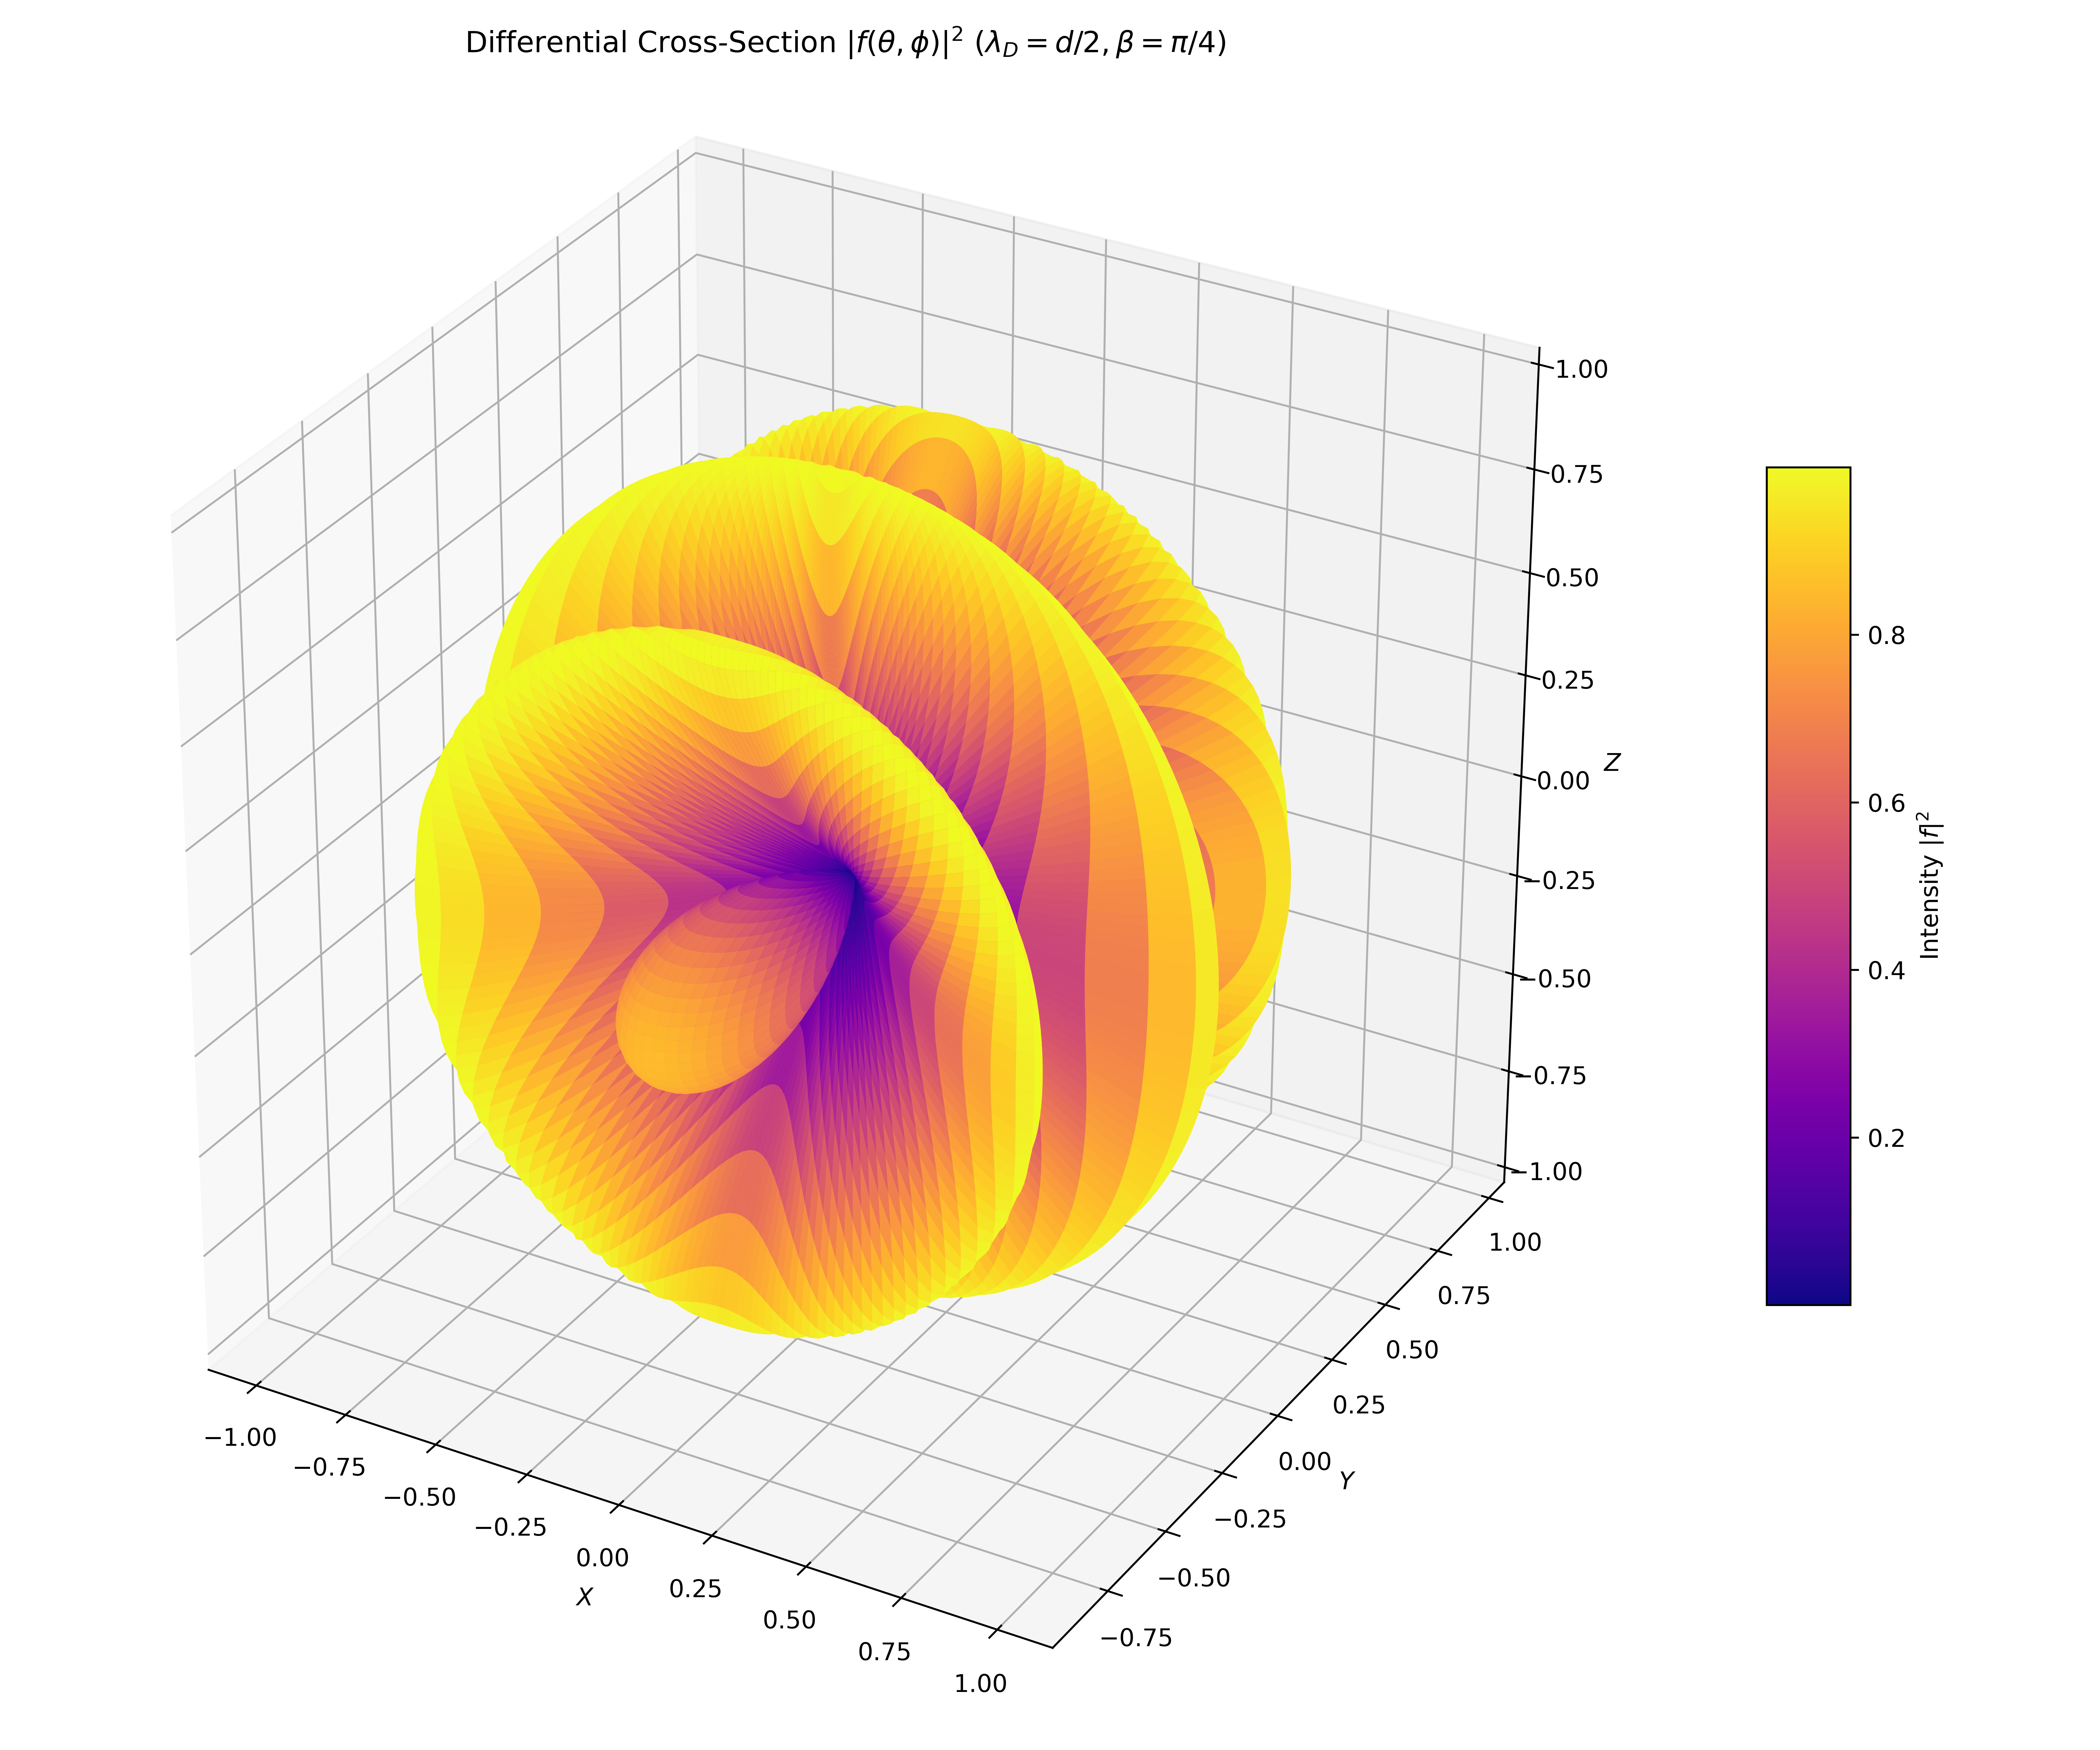
\includegraphics[scale=0.5]{../figures/scattering_cross_section.png}
	\caption{Surface plot of the differential scattering cross-section $\left| f(\theta ,\phi ) \right| ^2$ for a neutron scattered by two delta functions in the first Born approximation.}
	\label{fig:1}
	\centering
\end{figure}
\newpage


\section{L3. Teleportation protocol EPR entangled state}

I will use the following notation, which heavily simplifies the annoying notation in this problem. I will write $\ket{0_i}\ket{0_A}\ket{0_B}$ as $\ket{000}$, and similarly for any 1s. I will only use this notation after fully distributing tensor over addition (which follows by bilinearity of tensor), since doing it before can be confusing, but there is no possibility for confusion after, and it significantly cleans up notation in my opinion.

(a) We have
\[
	\ket{\Psi _{iAB} }=\ket{\phi _i}\otimes \ket{\Psi _{AB} }=\left( \alpha \ket{0_i}+ \beta \ket{1_i}\right) \otimes \frac{1}{\sqrt{2} } \left( \ket{0}\otimes \ket{1}+\ket{1}\otimes \ket{0} \right) 
\]
\[
	=\frac{\alpha }{\sqrt{2} } \ket{001}+\frac{\alpha }{\sqrt{2} } \ket{010}+\frac{\beta }{\sqrt{2} } \ket{101}+\frac{\beta }{\sqrt{2} } \ket{110}
.\]
Now acting on this by $U_{\mathrm{CNOT} } \otimes 1$:
\[
	\left( U_{\mathrm{CNOT} } \otimes 1 \right) \ket{\Psi _{iAB} }=\frac{\alpha }{\sqrt{2} } \left( U_{\mathrm{CNOT} } \ket{00}\otimes \ket{1} + U_{\mathrm{CNOT} } \ket{01}\otimes \ket{0} \right) +\frac{\beta }{\sqrt{2}} \left( U_{\mathrm{CNOT} } \ket{10}\otimes \ket{1}+U_{\mathrm{CNOT} } \ket{11}\otimes \ket{0} \right) 
.\]
We compute CNOT on each of the four 2-tensors. Recall the matrix representations of the relevant statevectors. We have
\[
	U_{\mathrm{CNOT} } \ket{00}=\begin{pmatrix}
	1 & 0 & 0 & 0 \\
	0 & 1 & 0 & 0 \\
	0 & 0 & 0 & 1 \\
	0 & 0 & 1 & 0
	\end{pmatrix}\begin{pmatrix}
	1 \\
	0 \\
	0 \\
	0
	\end{pmatrix}=\begin{pmatrix}
	1 \\
	0 \\
	0 \\
	0
\end{pmatrix}=\ket{00}
\]
\[
	U_{\mathrm{CNOT} } \ket{01}=\begin{pmatrix}
	1 & 0 & 0 & 0 \\
	0 & 1 & 0 & 0 \\
	0 & 0 & 0 & 1 \\
	0 & 0 & 1 & 0
	\end{pmatrix}\begin{pmatrix}
	0 \\
	1 \\
	0 \\
	0
	\end{pmatrix}=\begin{pmatrix}
	0 \\
	1 \\
	0 \\
	0
\end{pmatrix}=\ket{01}
\]
\[
	U_{\mathrm{CNOT} } \ket{10}=\begin{pmatrix}
	1 & 0 & 0 & 0 \\
	0 & 1 & 0 & 0 \\
	0 & 0 & 0 & 1 \\
	0 & 0 & 1 & 0
	\end{pmatrix}\begin{pmatrix}
	0 \\
	0 \\
	1 \\
	0
	\end{pmatrix}=\begin{pmatrix}
	0 \\
	0 \\
	0 \\
	1
\end{pmatrix}=\ket{11}
\]
\[
	U_{\mathrm{CNOT} } \ket{11}=\begin{pmatrix}
	1 & 0 & 0 & 0 \\
	0 & 1 & 0 & 0 \\
	0 & 0 & 0 & 1 \\
	0 & 0 & 1 & 0
	\end{pmatrix}\begin{pmatrix}
	0 \\
	0 \\
	0 \\
	1
	\end{pmatrix}=\begin{pmatrix}
	0 \\
	0 \\
	1 \\
	0
\end{pmatrix}=\ket{10}.
\]
Thus
\[
	\left( U_{\mathrm{CNOT} } \otimes 1 \right) \ket{\Psi _{iAB} }=\frac{\alpha }{\sqrt{2} } \ket{001}+\frac{\alpha }{\sqrt{2} } \ket{010}+\frac{\beta }{\sqrt{2} } \ket{111}+\frac{\beta }{\sqrt{2} } \ket{100}
.\]

(b) Performing the Hadamard transformation $\hat{H} \otimes 1\otimes 1$:
\[
	\left( \hat{H} \otimes 1\otimes 1 \right) \ket{\Psi _{iAB} }=\frac{\alpha }{\sqrt{2} } \left( \hat{H}\ket{0}\otimes \ket{01}+ \hat{H} \ket{0}+\ket{10} \right) +\frac{\beta }{\sqrt{2} } \left( \hat{H} \ket{1}\otimes \ket{11}+ \hat{H} \ket{1}\otimes \ket{00} \right) 
.\]
We compute the Hadamard on both qubit states:
\[
	\hat{H} \ket{0} = \frac{1}{\sqrt{2} } \begin{pmatrix}
	1 & 1 \\
	1 & -1
	\end{pmatrix}\begin{pmatrix}
	1 \\
	0
	\end{pmatrix}=\frac{1}{\sqrt{2} } \begin{pmatrix}
	1 \\
	1
\end{pmatrix}=\frac{1}{\sqrt{2} } \left( \ket{0}+\ket{1} \right) 
\]
\[
	\hat{H} \ket{1}=\frac{1}{\sqrt{2} }\begin{pmatrix}
	1 & 1 \\
	1 & -1
	\end{pmatrix}\begin{pmatrix}
	0 \\
	1
	\end{pmatrix}=\frac{1}{\sqrt{2} } \begin{pmatrix}
	1 \\
	-1
\end{pmatrix}=\frac{1}{\sqrt{2} } \left( \ket{0}-\ket{1} \right) 
.\]
Plugging in and distributing over tensor yields
\[
	\left( \hat{H} \otimes 1\otimes 1 \right) \ket{\Psi _{iAB} }=\frac{\alpha }{2} \left( \ket{001}+\ket{101}+\ket{010}+\ket{110} \right) +\frac{\beta }{2} \left( \ket{011}-\ket{111}+\ket{000}-\ket{100} \right) 
.\]
Note that all of these terms are distinct. It will be useful for the final part to put this in the form given in the question. This is equal to
\[
.\]
\begin{align*}
	(\hat{H} \otimes 1\otimes 1)\ket{\Psi _{iAB} }=\,\,&\ket{00}\left( \frac{\alpha }{2} \ket{1}+\frac{\beta }{2} \ket{0} \right) +\\
							   &\ket{01}\left( \frac{\alpha }{2} \ket{0} +\frac{\beta }{2} \ket{1}\right) +\\
							   &\ket{10}\left( -\frac{\beta }{2} \ket{0}+\frac{\alpha }{2} \ket{1} \right) \\
							   &\ket{11}\left( \frac{\alpha }{2} \ket{0}-\frac{\beta }{2} \ket{1} \right) 
.\end{align*}


(c) Alice's qubits are the first two numbers, and Bob's qubit is the final number in the above expansion. We can read the results directly off of the above expression. The operators are justified below. Note that the factor of $1/2$ vanishes when we measure the first two qubits since the resultant qubit must be normalized (we can specifically pull out a $1/2$ rather than some other combination of coefficients since any other possibility varies only by a global phase factor). 
\begin{center}
\begin{tabular}{|c|c|c|c|}
	\hline
	Alice measures & Bob's qubit collapses to & Bob uses operator & Desired outcome\\
	\hline
	$\ket{00}$ & $\alpha \ket{1}+\beta \ket{0}$ & $\sigma _x$ & $\alpha \ket{0}+\beta \ket{1}$\\
	\hline
	$\ket{01}$ & $\alpha \ket{0}+\beta \ket{1}$ & 1 & $\alpha \ket{0}+\beta \ket{1}$\\
	\hline
	$\ket{10}$ & $-\beta \ket{0}+\alpha \ket{1}$ & $\sigma _z\sigma _x$ & $\alpha \ket{0}+\beta \ket{1}$\\
	\hline
	$\ket{11}$ & $\alpha \ket{0}-\beta \ket{1}$ & $\sigma _z$ & $\alpha \ket{0}+\beta \ket{1}$\\
	\hline
\end{tabular}
\end{center}
Justifying the operators is simple. Recall the very easily shown identities
\[
	\sigma _x\ket{0}=\ket{1},\qquad \sigma _x\ket{1}=\ket{0},\qquad \sigma _z\ket{0}=\ket{0},\qquad \sigma _z\ket{1}=-\ket{1}
.\]
In case 1, we have
\[
	\sigma _x\left( \alpha \ket{1}+\beta \ket{0} \right) =\alpha \sigma _x\ket{1}+\beta \sigma _x\ket{0}=\alpha \ket{0}+\beta \ket{1}
.\]
In case 2, the state is already the desired state. In case 3,
\[
	\sigma _x\left( -\beta \ket{0}+\alpha \ket{1} \right) =-\beta \sigma _x\ket{0}+\alpha \sigma _x\ket{1}=\alpha \ket{0}-\beta \ket{1}
.\]
This reduces case 3 to case 4. We then have
\[
	\sigma _z\left( \alpha \ket{0}-\beta \ket{1} \right) =\alpha \sigma _z\ket{0}-\beta \sigma _z\ket{1}=\alpha \ket{0}+\beta \ket{1}
.\]



\end{document}
